\chapter{Signal injection results}
% \markboth{}{Appendix A}
\label{app:si_results}


\paragraph{Gaussian signals}

In \Figrange{\ref{fig:si_results:siginj_gaus_SR}}{\ref{fig:si_results:siginj_gaus_SRB}}, results of the \ac{SI} test with Gaussian signals are shown for the different gaussian widths of \(\sigma_G/\mG = 0.02, \, 0.05\) and \(0.20\). The tests have been carried out in each one of the analysis regions using the Gaussian signal model: SR, SRL, SRC and SRB. For all widths hypothesis the test is passed as linear behaviours are seen, and the ratio of \(\left|\sspur\right| / N_{\text{inj}} < 0.5\) 


\begin{figure}[ht!]
    \centering
    \begin{subfigure}[h]{0.32\linewidth}
        \centering
        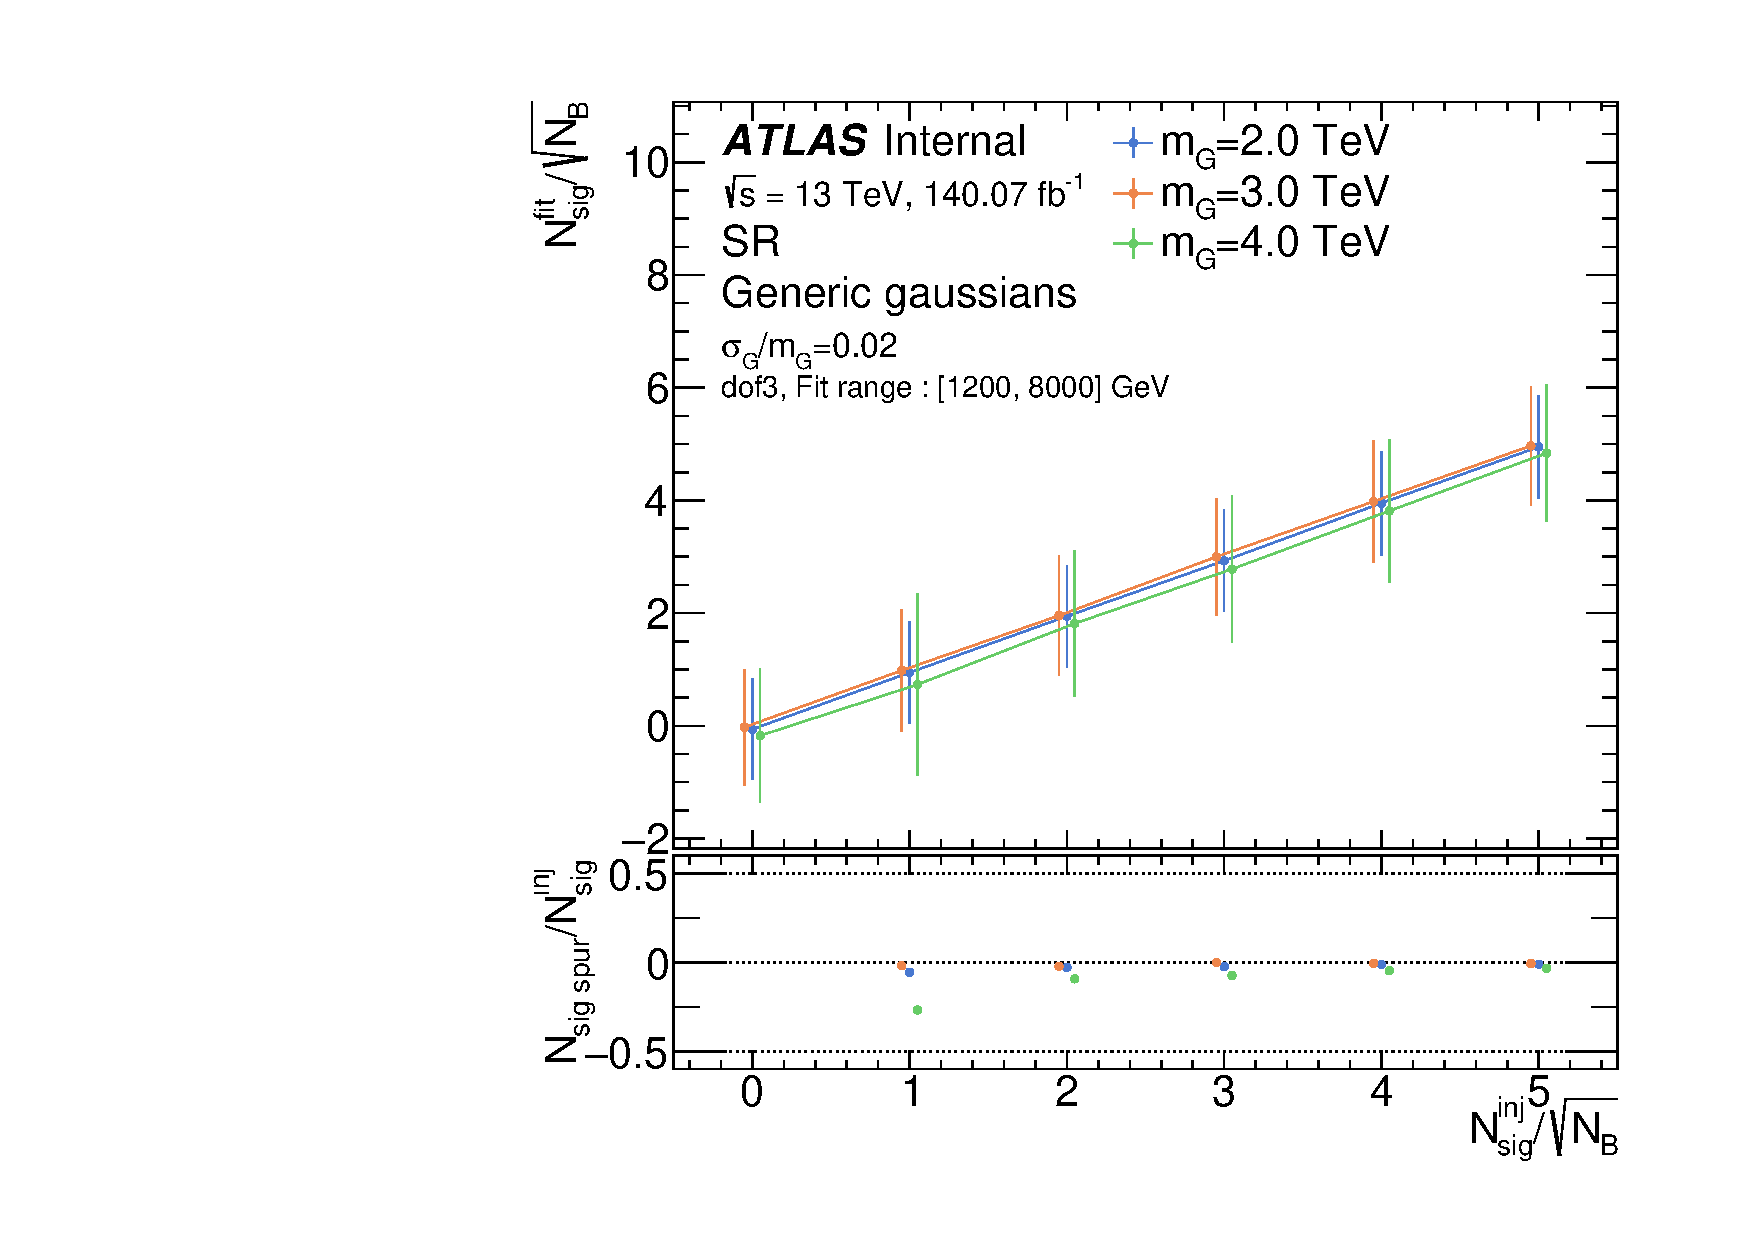
\includegraphics[width=\textwidth]{5_resonances/bkg/modeling/si/toys/SR/gaus/width0p02/dof3__range_1200_8000/plots/can__SigInj__photonjet_Pythia_jfakeisosmooth__gaus__SR__width0p02__dof3__range_1200_8000}
        \caption{\(\sigma_G/\mG = 0.02\).}
    \end{subfigure}
    \hfill
    \begin{subfigure}[h]{0.32\linewidth}
        \centering
        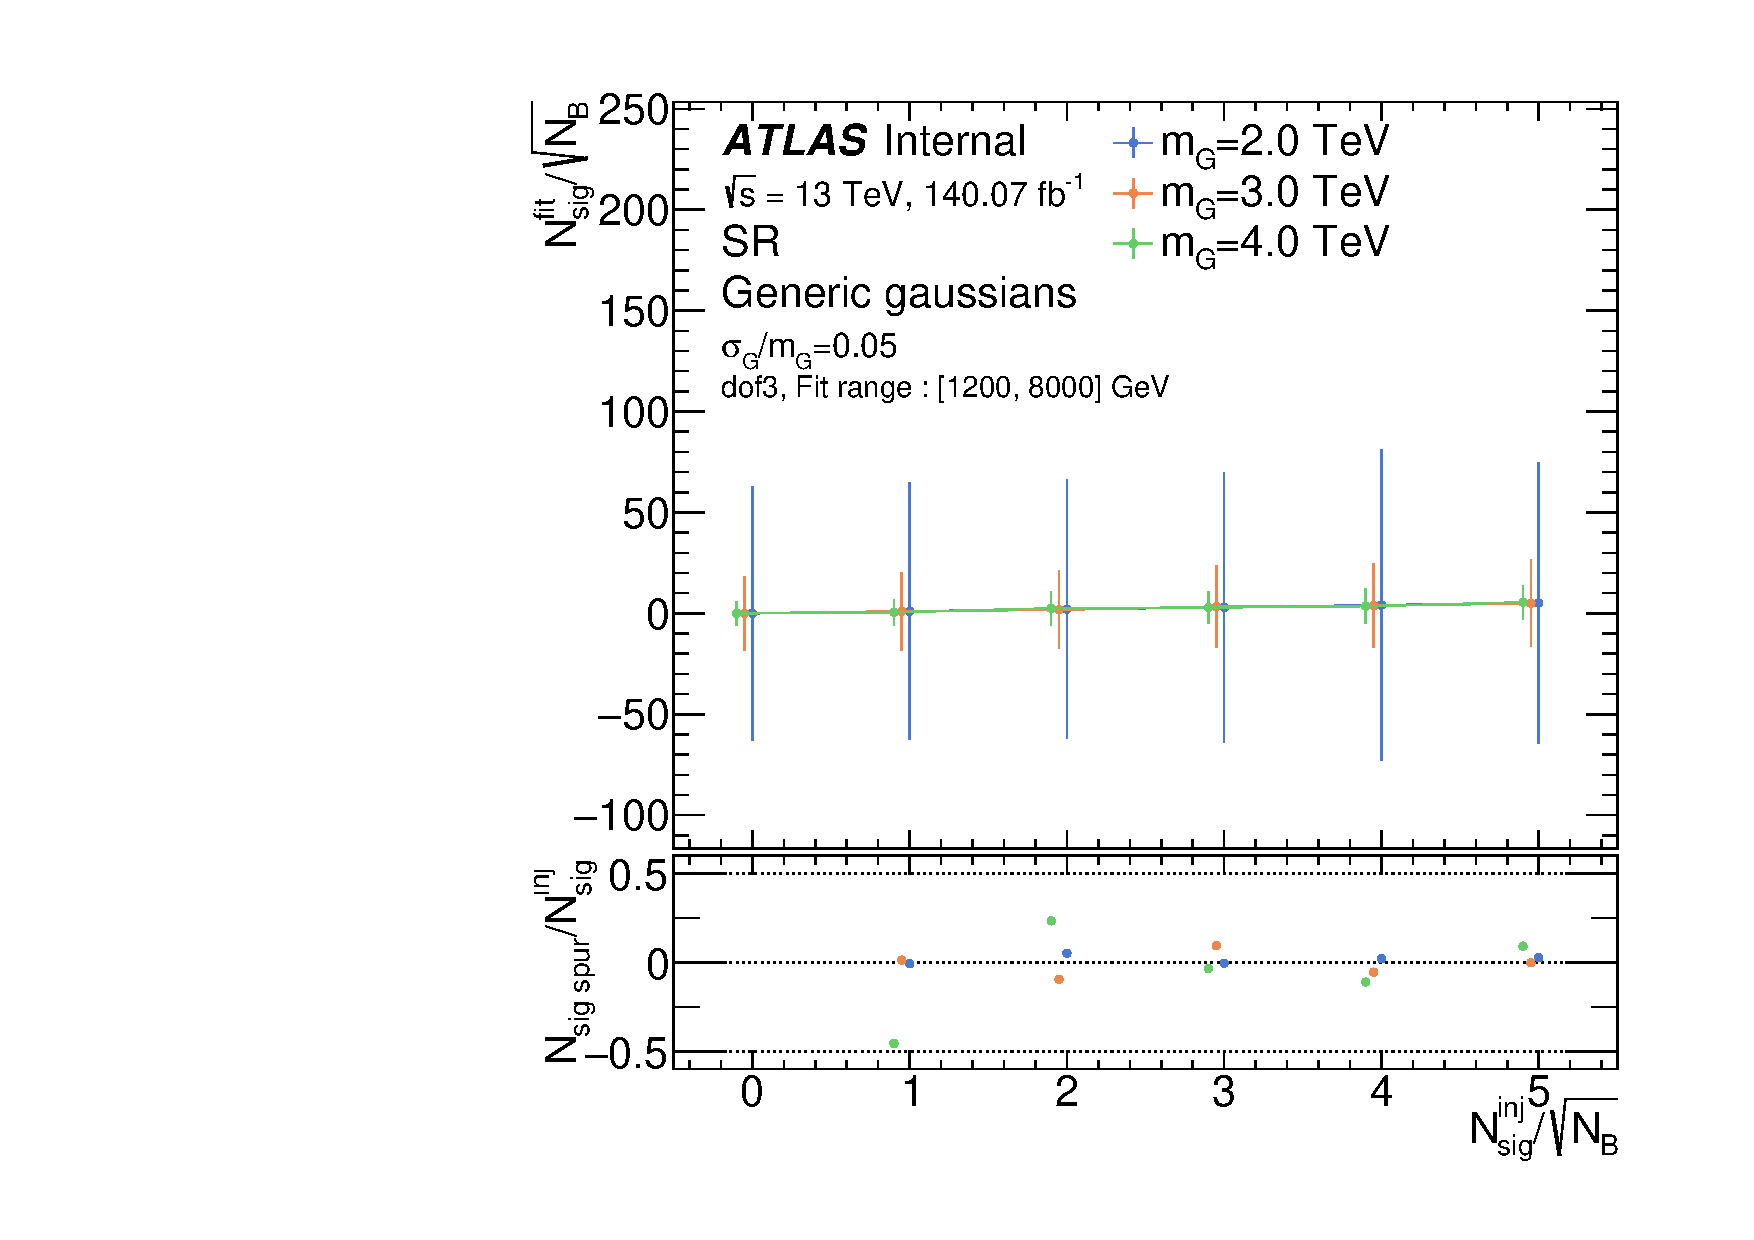
\includegraphics[width=\textwidth]{5_resonances/bkg/modeling/si/toys/SR/gaus/width0p05/dof3__range_1200_8000/plots/can__SigInj__photonjet_Pythia_jfakeisosmooth__gaus__SR__width0p05__dof3__range_1200_8000}
        \caption{\(\sigma_G/\mG = 0.05\).}
    \end{subfigure}
    \hfill
    \begin{subfigure}[h]{0.32\linewidth}
        \centering
        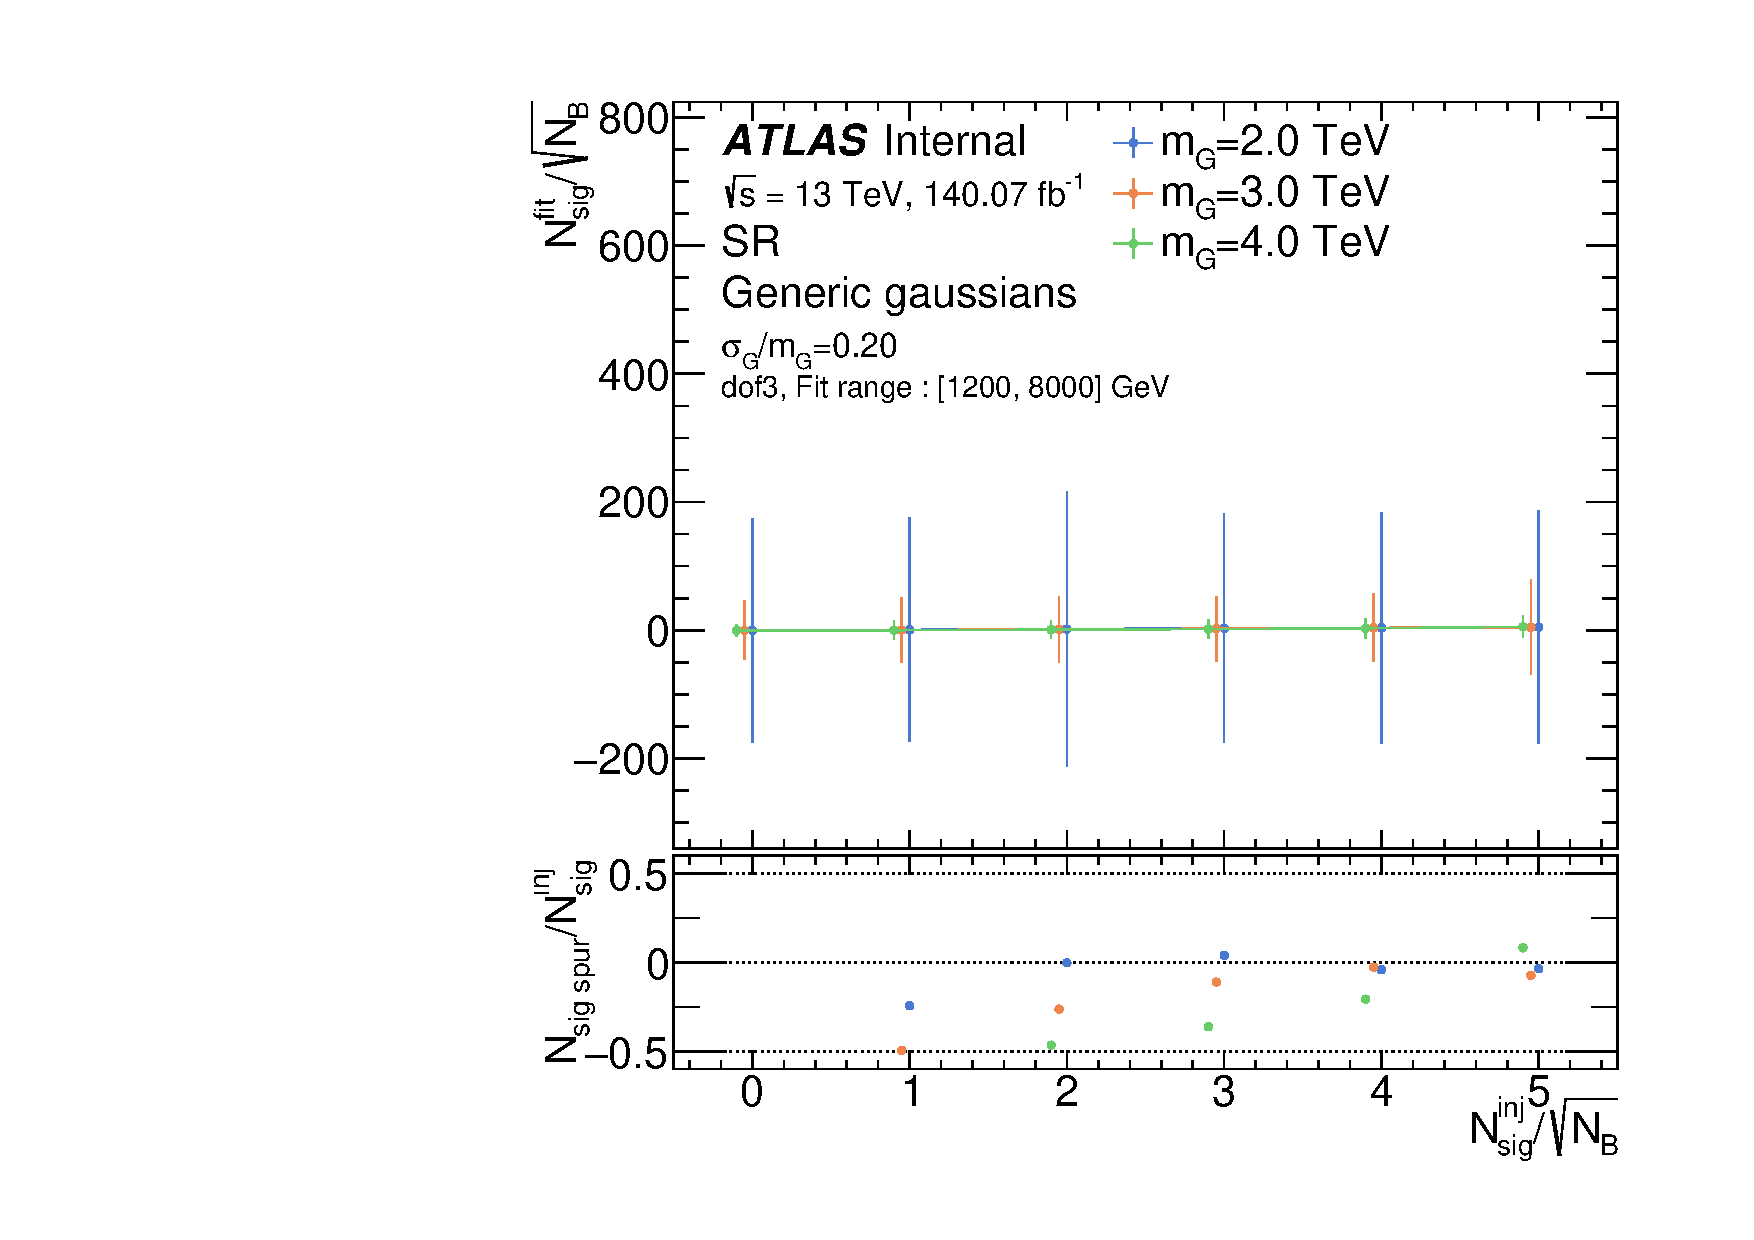
\includegraphics[width=\textwidth]{5_resonances/bkg/modeling/si/toys/SR/gaus/width0p20/dof3__range_1200_8000/plots/can__SigInj__photonjet_Pythia_jfakeisosmooth__gaus__SR__width0p20__dof3__range_1200_8000}
        \caption{\(\sigma_G/\mG = 0.20\).}
    \end{subfigure}
    \caption{\ac{SI} tests results using Gaussians signals in the inclusive SR region. The fit is performed in the range \(1200-8000~\gev\) using the \textit{dof3} function. Each considered mass is shown with a different color. The \(x\)-axis shows the injected amplitude in units of \(\sqrt{N_B}\), while the \(y\)-axis represents the extracted signal in terms of \(\sqrt{N_B}\).}
    \label{fig:si_results:siginj_gaus_SR}
\end{figure}

\begin{figure}[ht!]
    \centering
    \begin{subfigure}[h]{0.32\linewidth}
        \centering
        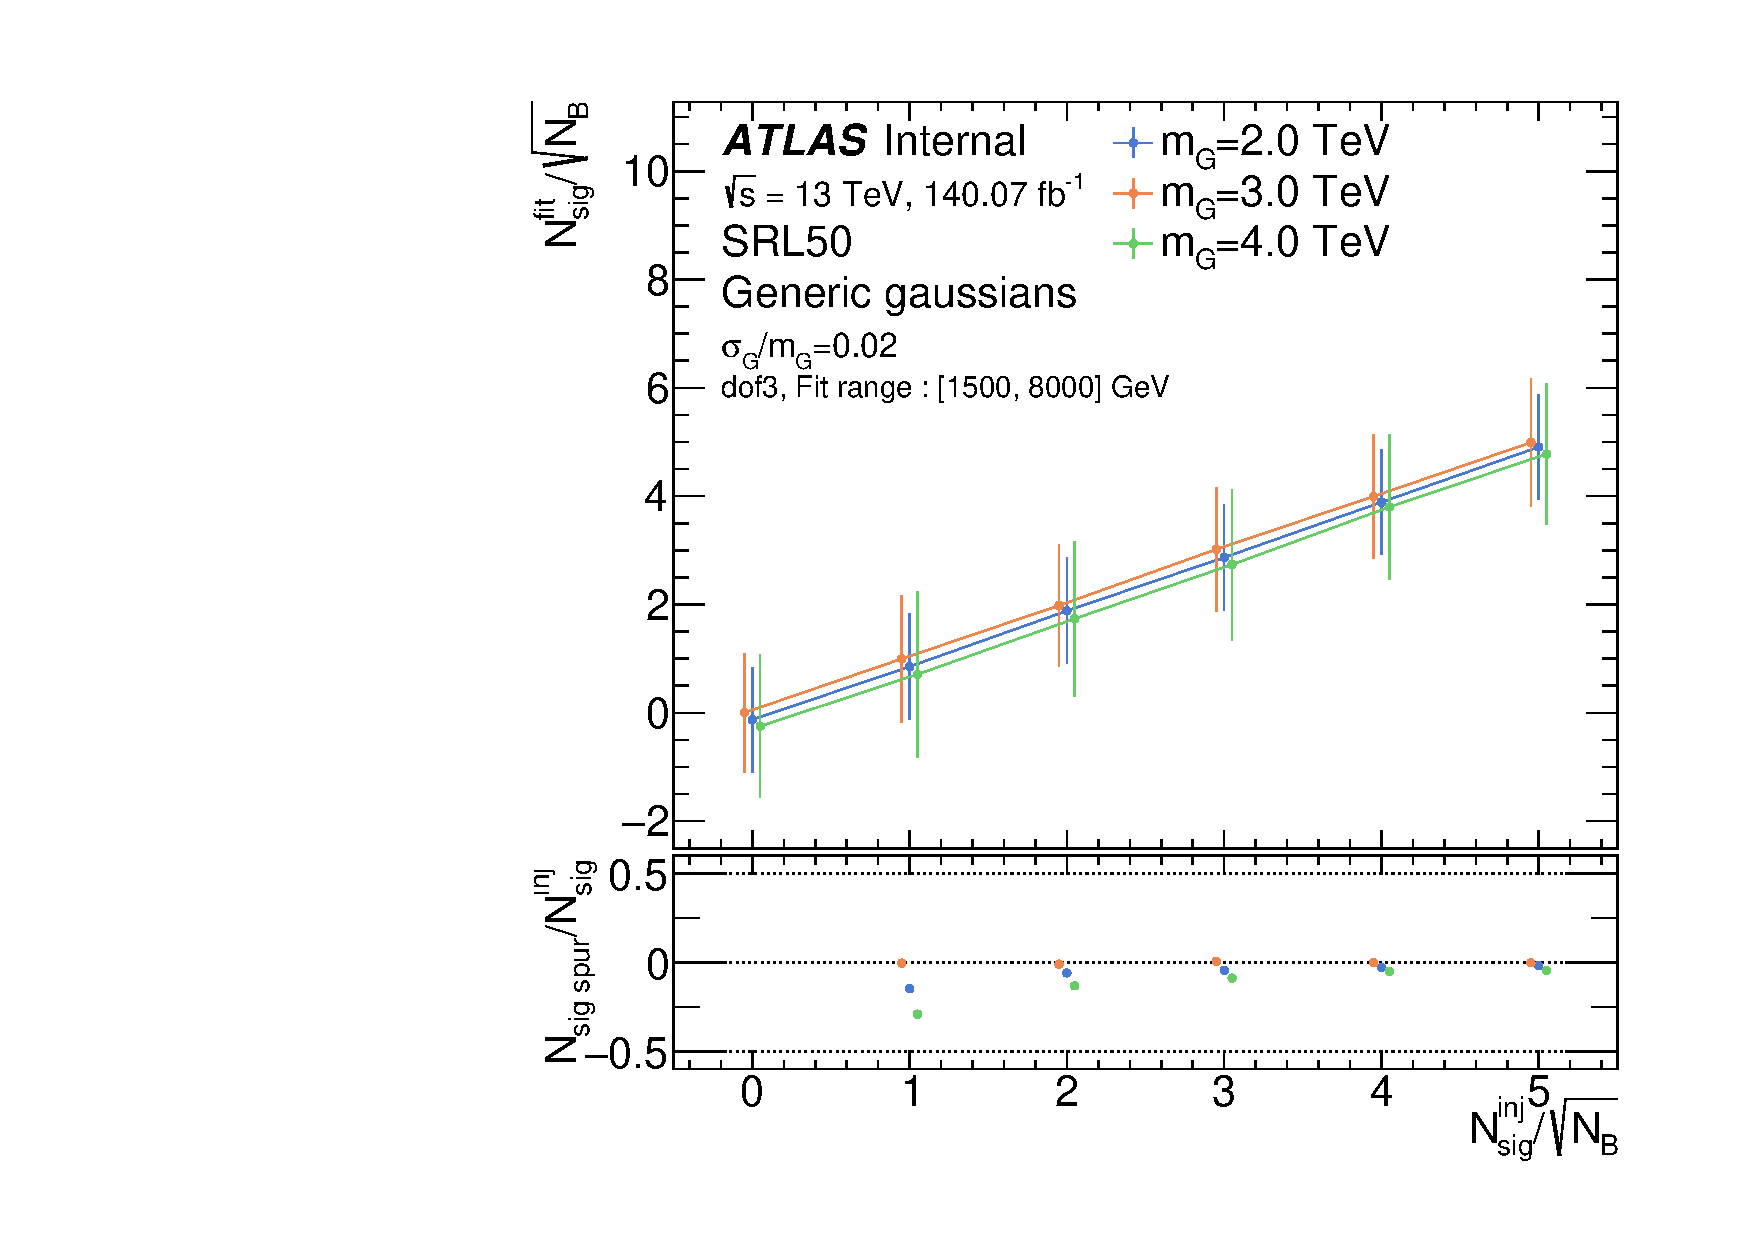
\includegraphics[width=\textwidth]{5_resonances/bkg/modeling/si/toys/SRL50/gaus/width0p02/dof3__range_1500_8000/plots/can__SigInj__photonjet_Pythia_jfakeisosmooth__gaus__SRL50__width0p02__dof3__range_1500_8000}
        \caption{\(\sigma_G/\mG = 0.02\).}
    \end{subfigure}
    \hfill
    \begin{subfigure}[h]{0.32\linewidth}
        \centering
        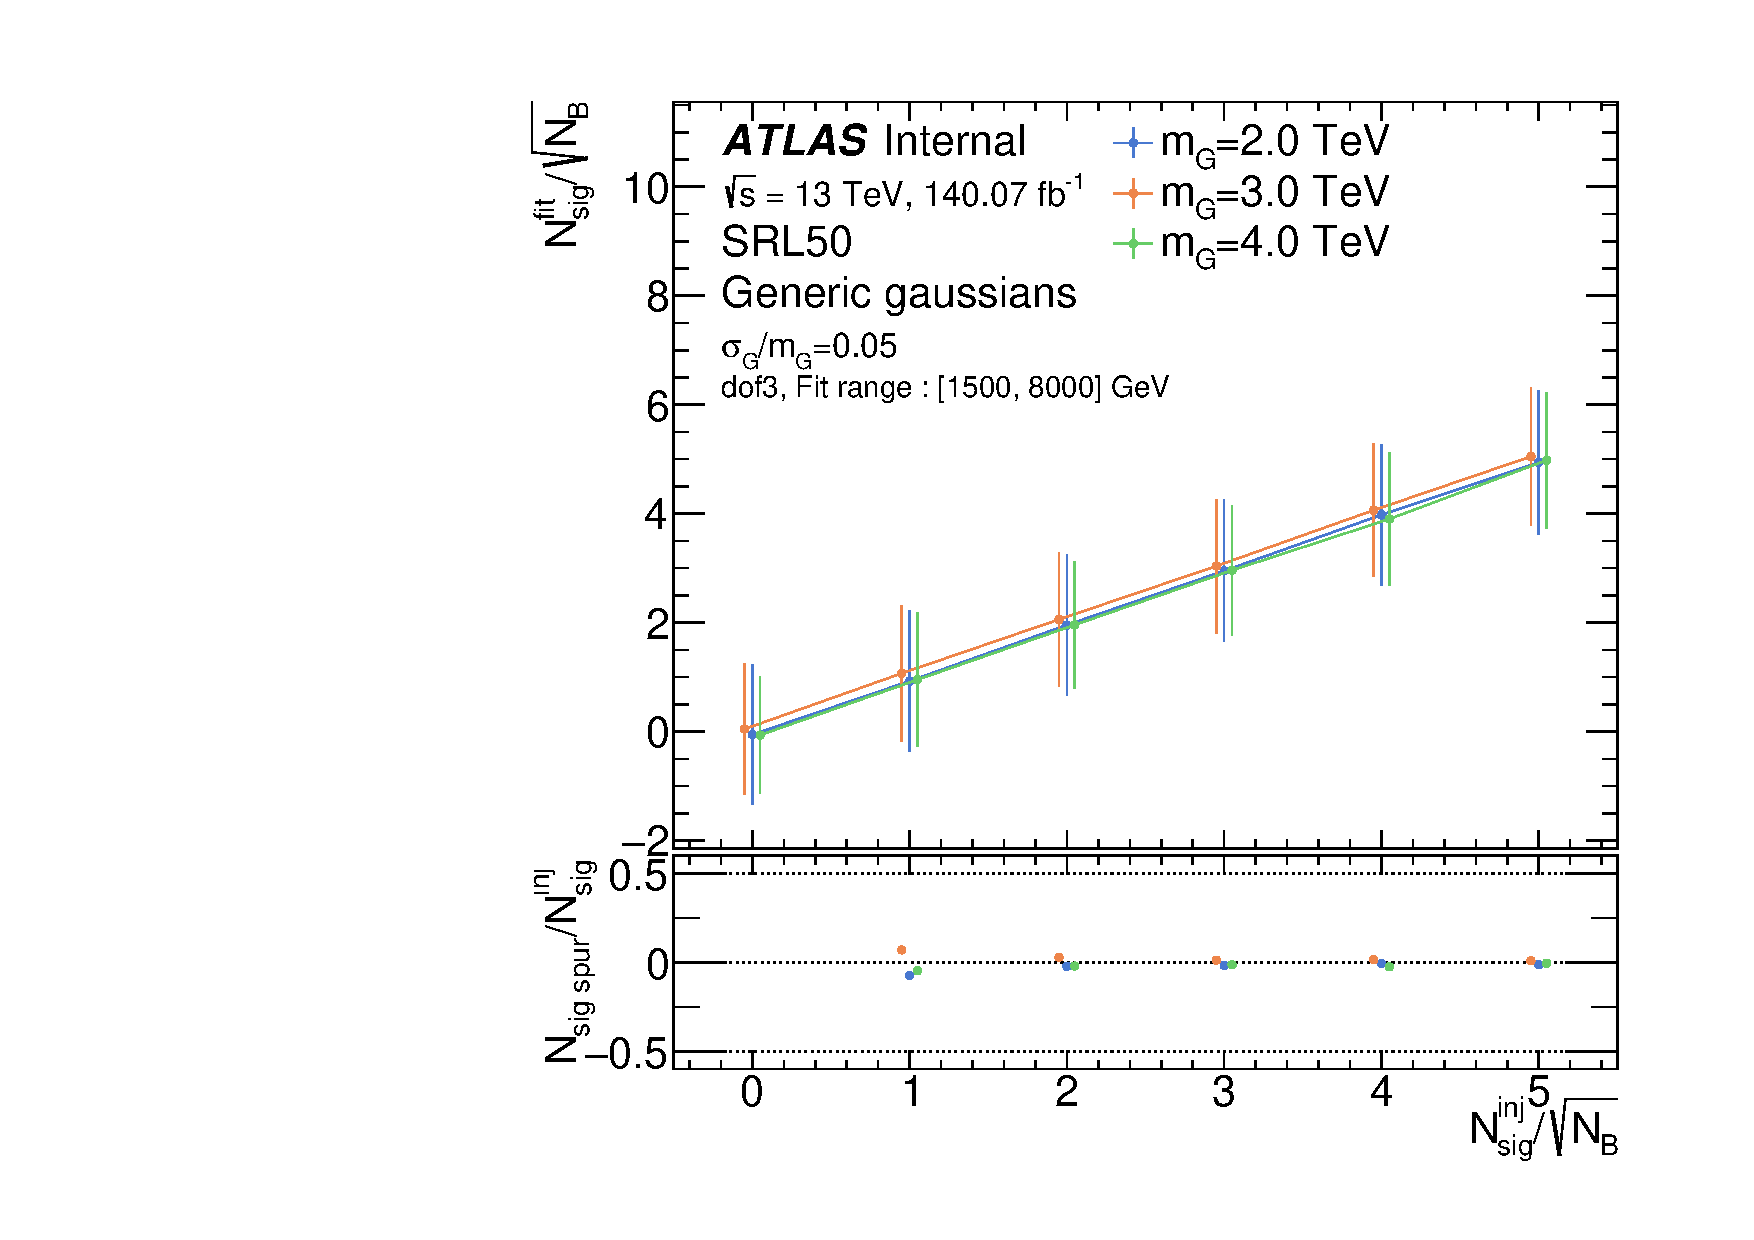
\includegraphics[width=\textwidth]{5_resonances/bkg/modeling/si/toys/SRL50/gaus/width0p05/dof3__range_1500_8000/plots/can__SigInj__photonjet_Pythia_jfakeisosmooth__gaus__SRL50__width0p05__dof3__range_1500_8000}
        \caption{\(\sigma_G/\mG = 0.05\).}
    \end{subfigure}
    \hfill
    \begin{subfigure}[h]{0.32\linewidth}
        \centering
        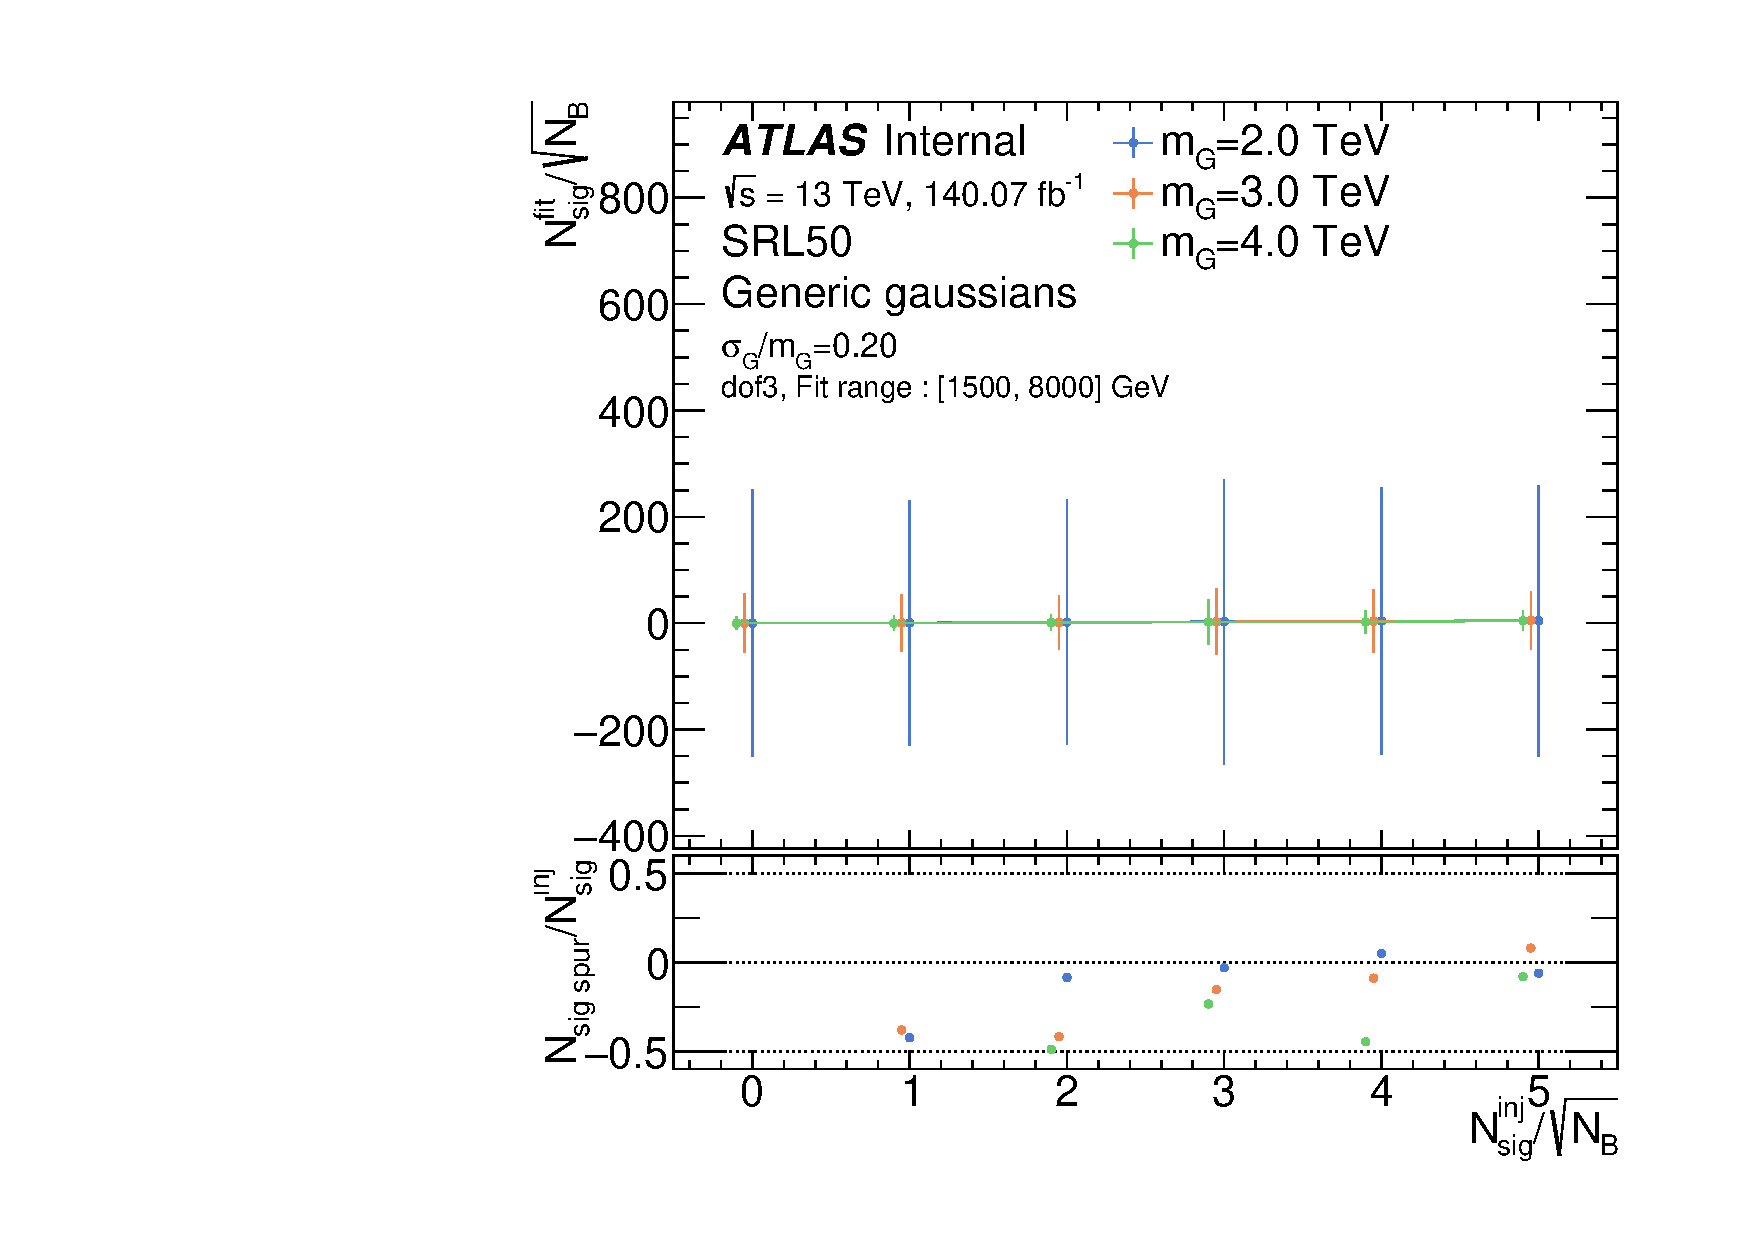
\includegraphics[width=\textwidth]{5_resonances/bkg/modeling/si/toys/SRL50/gaus/width0p20/dof3__range_1500_8000/plots/can__SigInj__photonjet_Pythia_jfakeisosmooth__gaus__SRL50__width0p20__dof3__range_1500_8000}
        \caption{\(\sigma_G/\mG = 0.20\).}
    \end{subfigure}
    \caption{Same as \Fig{\ref{fig:si_results:siginj_gaus_SR}} in the SRL region performing fits in the range \(1500-8000~\gev\) with the \textit{dpf3} function.}
    \label{fig:si_results:siginj_gaus_SRL}
\end{figure}

\begin{figure}[ht!]
    \centering
    \begin{subfigure}[h]{0.32\linewidth}
        \centering
        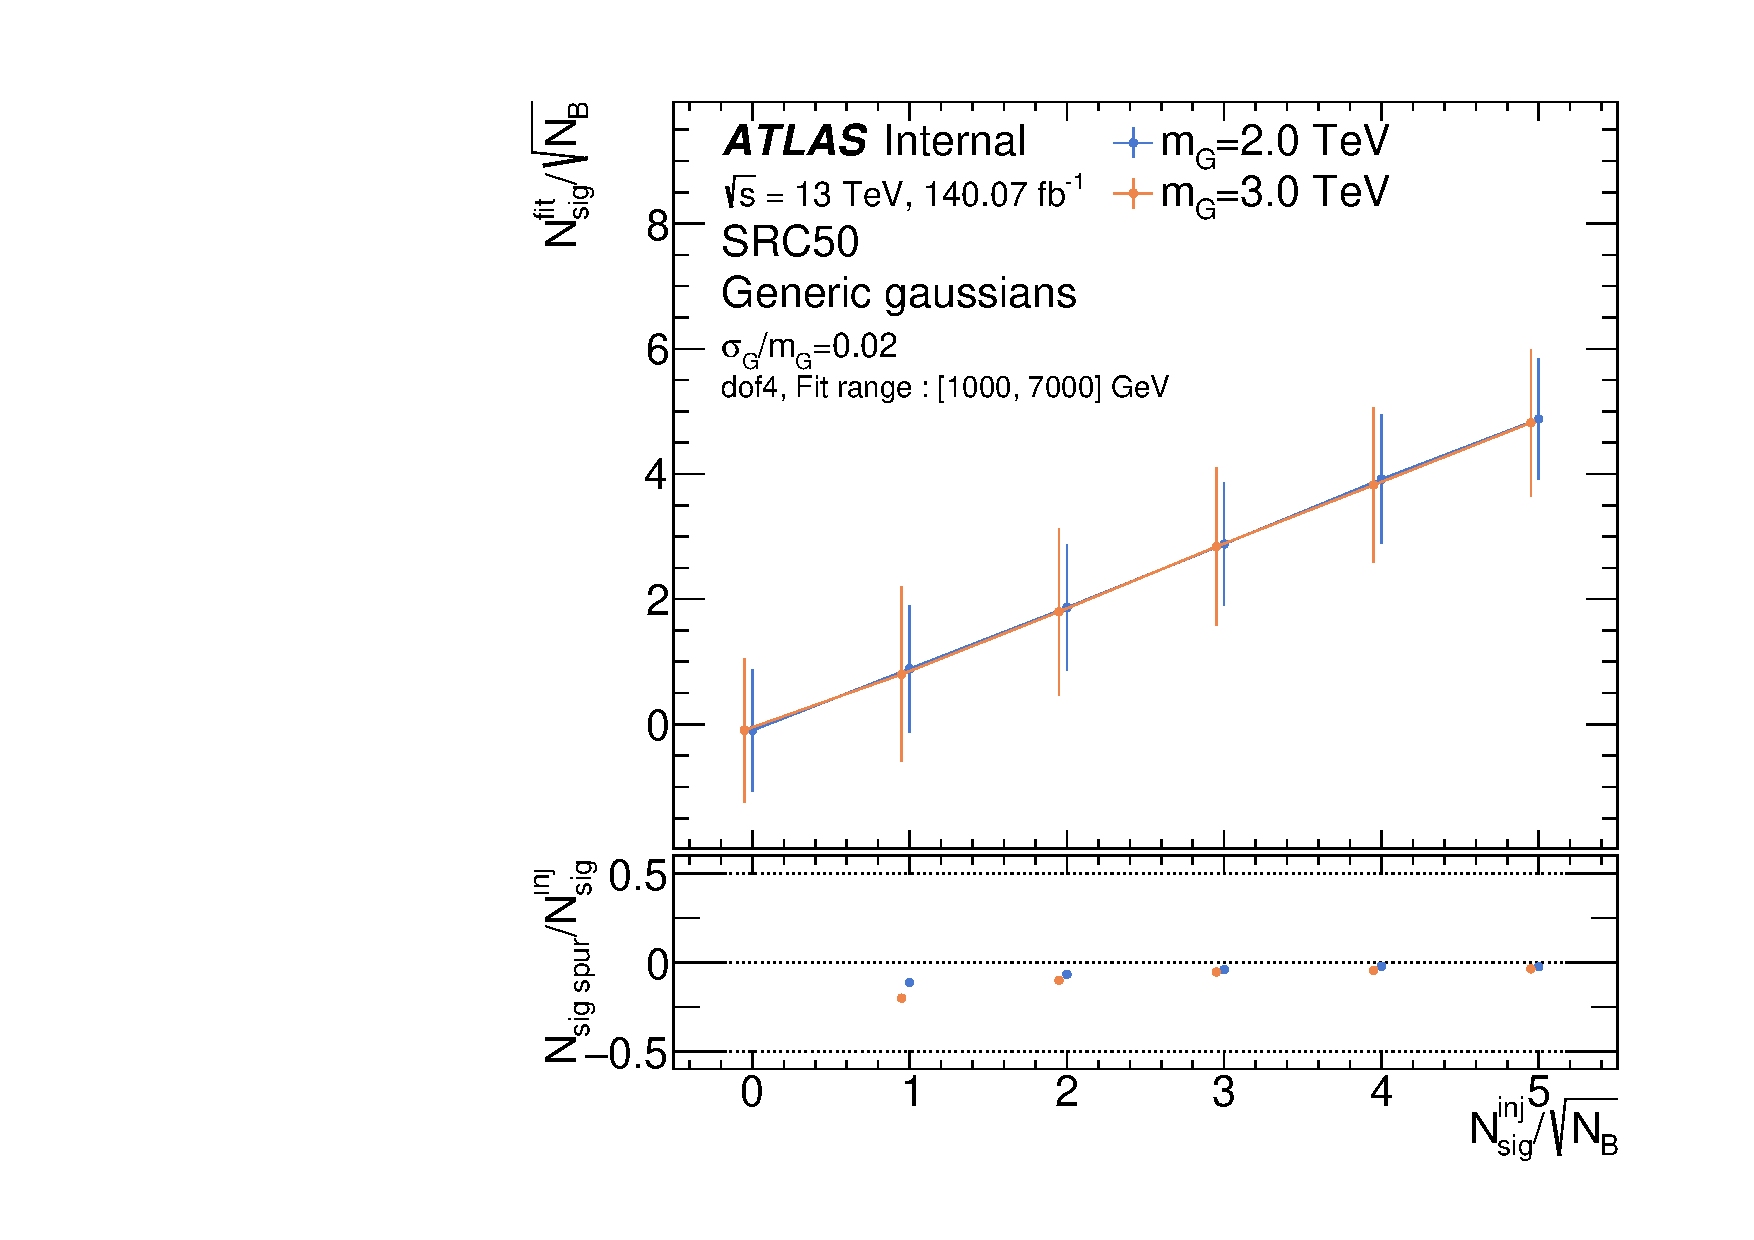
\includegraphics[width=\textwidth]{5_resonances/bkg/modeling/si/toys/SRC50/gaus/width0p02/dof4__range_1000_7000/plots/can__SigInj__photonjet_Pythia_jfakeisosmooth__gaus__SRC50__width0p02__dof4__range_1000_7000}
        \caption{\(\sigma_G/\mG = 0.02\).}
    \end{subfigure}
    \hfill
    \begin{subfigure}[h]{0.32\linewidth}
        \centering
        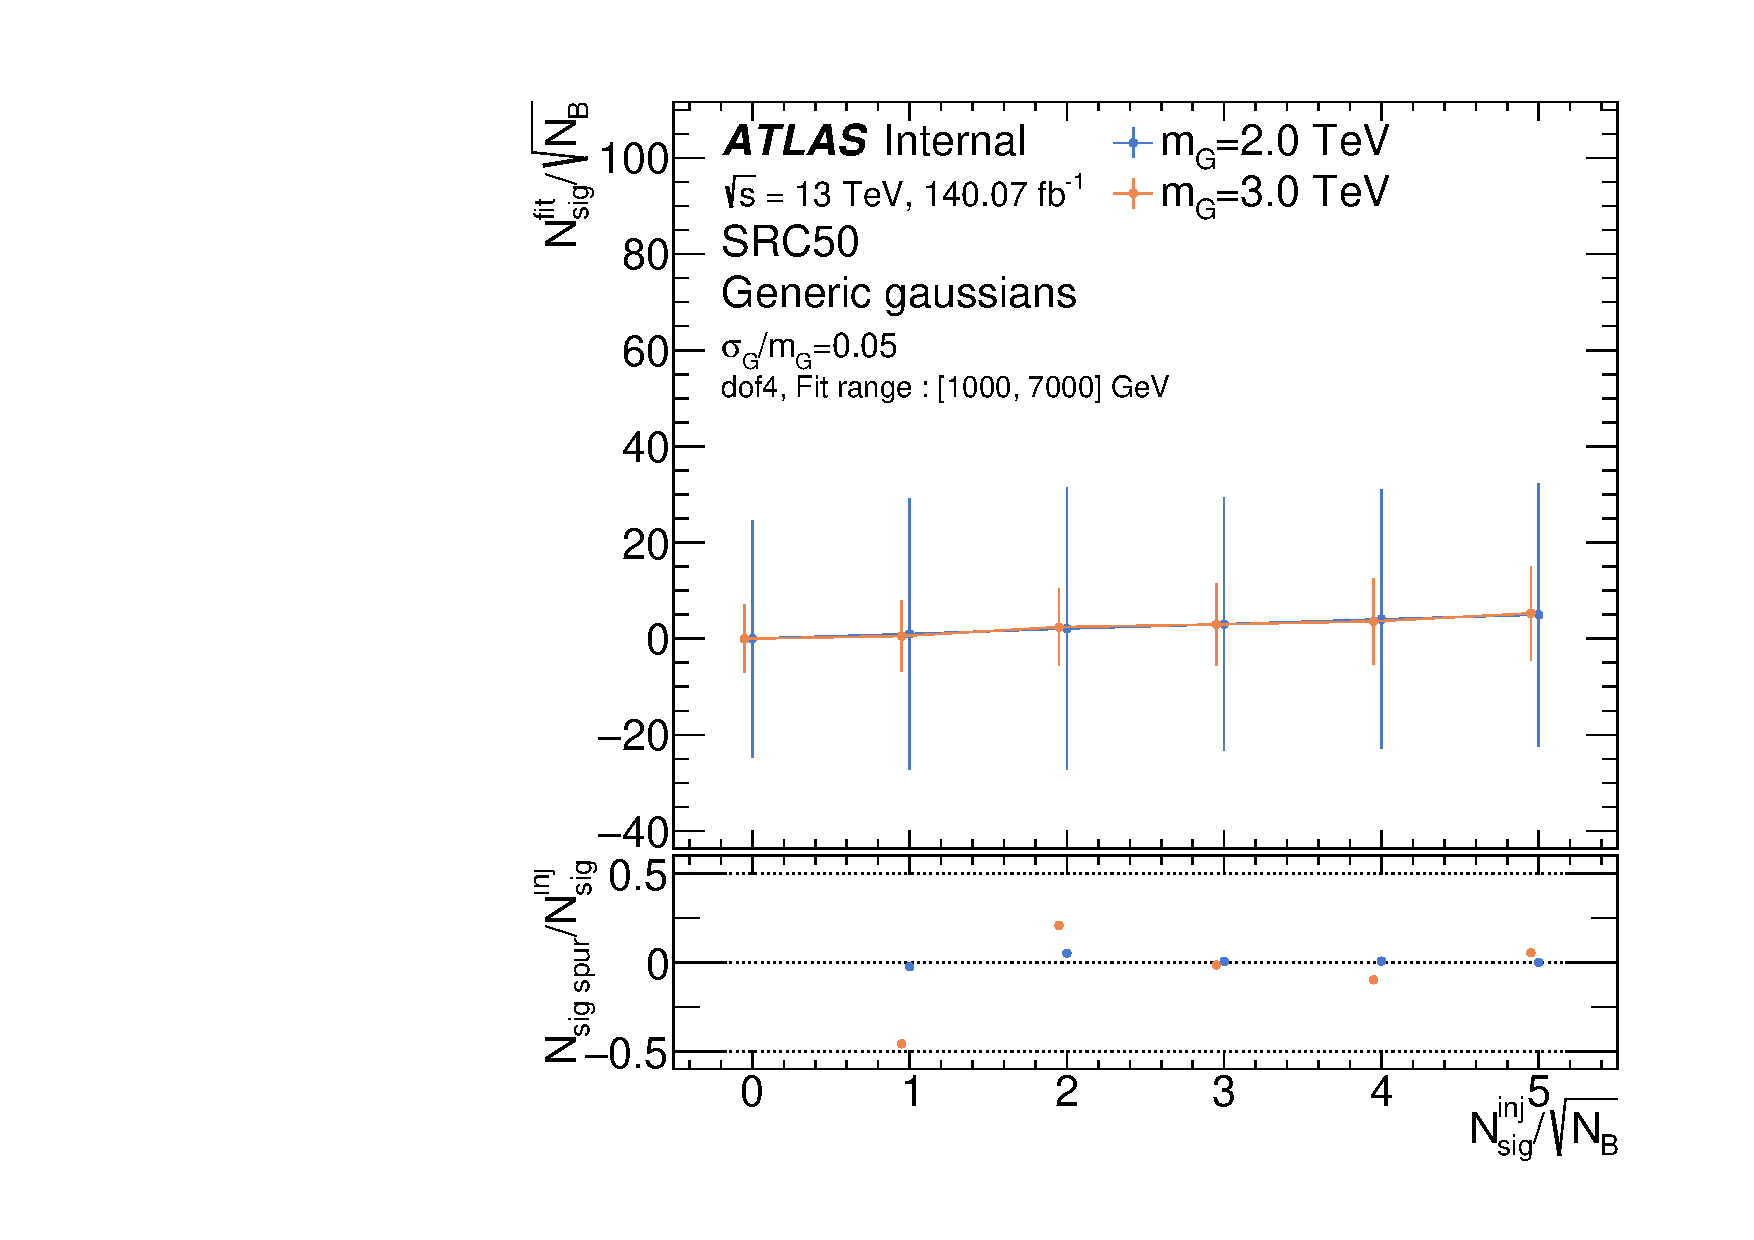
\includegraphics[width=\textwidth]{5_resonances/bkg/modeling/si/toys/SRC50/gaus/width0p05/dof4__range_1000_7000/plots/can__SigInj__photonjet_Pythia_jfakeisosmooth__gaus__SRC50__width0p05__dof4__range_1000_7000}
        \caption{\(\sigma_G/\mG = 0.05\).}
    \end{subfigure}
    \hfill
    \begin{subfigure}[h]{0.32\linewidth}
        \centering
        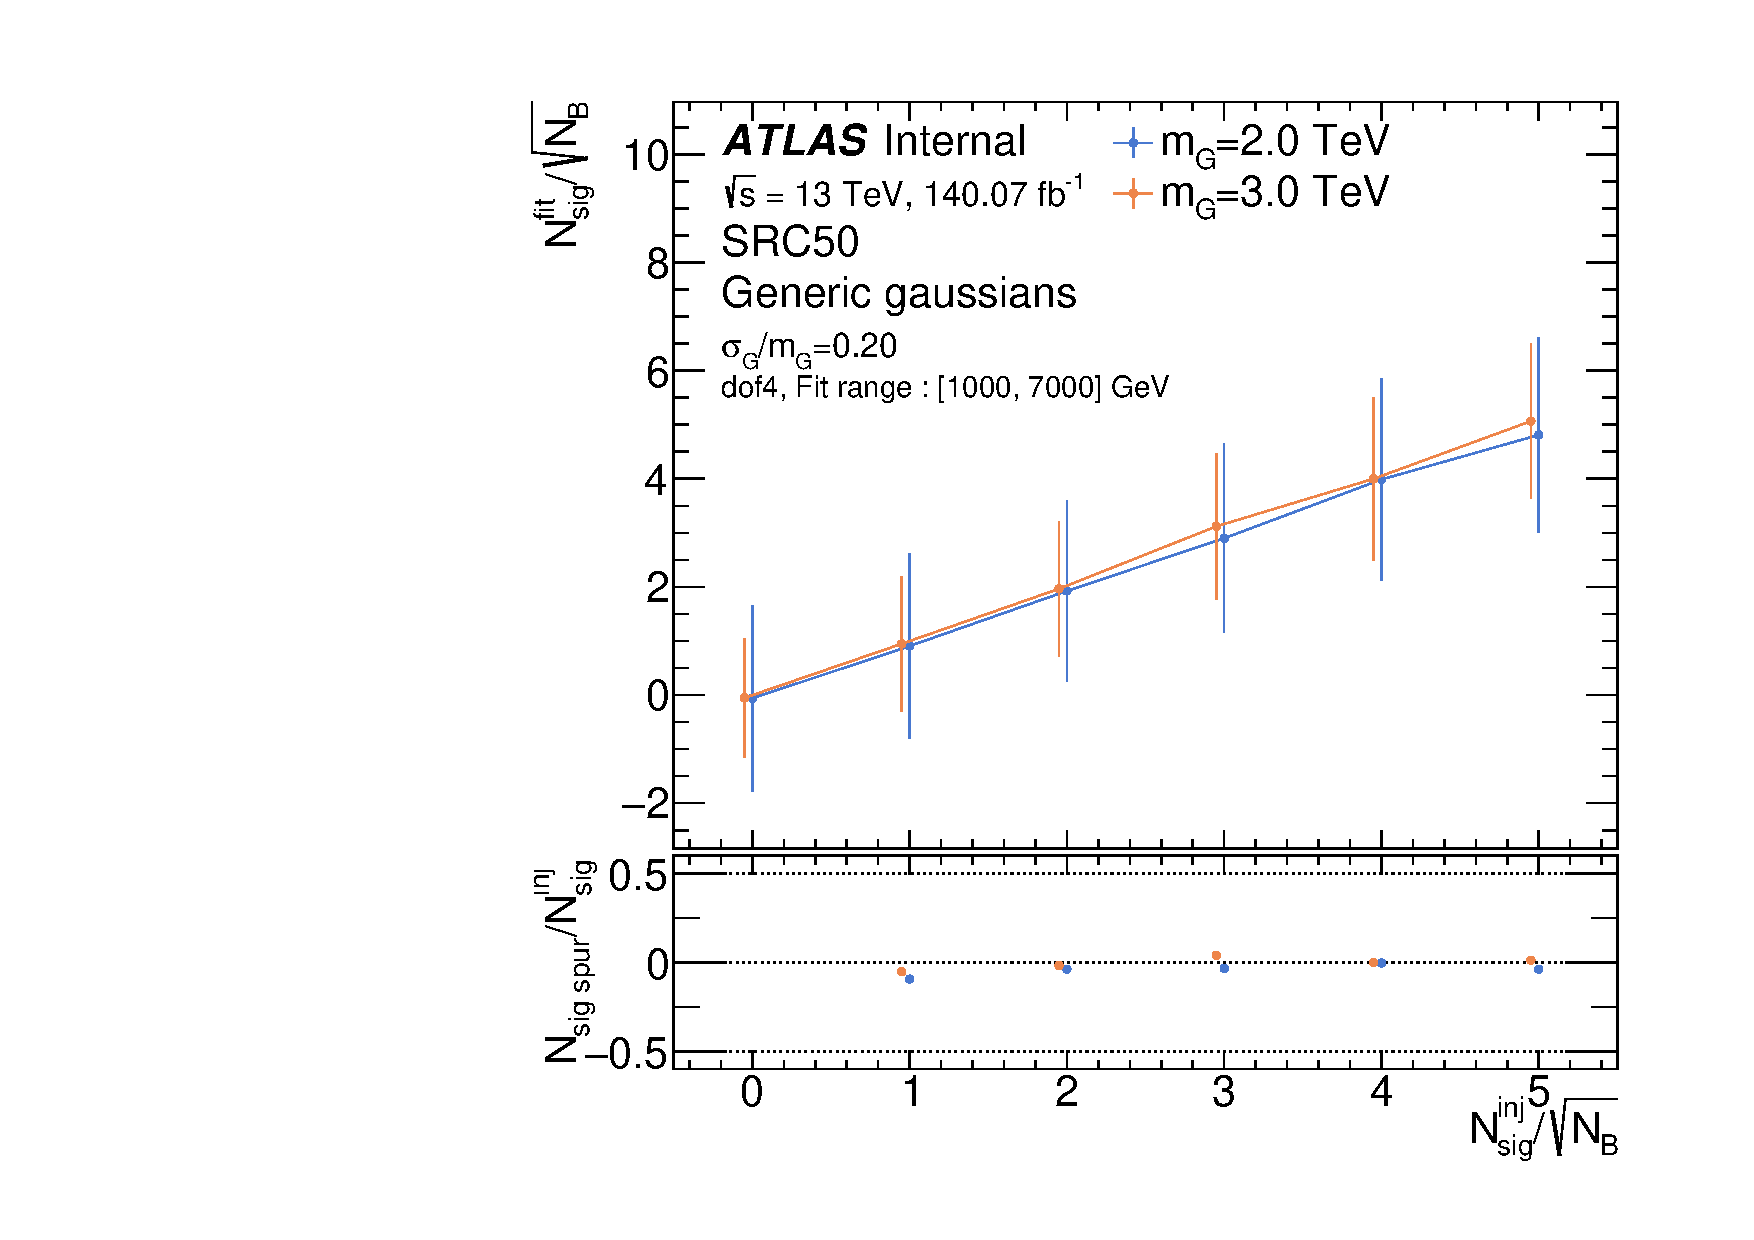
\includegraphics[width=\textwidth]{5_resonances/bkg/modeling/si/toys/SRC50/gaus/width0p20/dof4__range_1000_7000/plots/can__SigInj__photonjet_Pythia_jfakeisosmooth__gaus__SRC50__width0p20__dof4__range_1000_7000}
        \caption{\(\sigma_G/\mG = 0.20\).}
    \end{subfigure}
    \caption{Same as \Fig{\ref{fig:si_results:siginj_gaus_SR}} in the SRC region performing fits in the range \(1000-7000~\gev\) with the \textit{dpf4} function.}
    \label{fig:si_results:siginj_gaus_SRC}
\end{figure}

\begin{figure}[ht!]
    \centering
    \begin{subfigure}[h]{0.32\linewidth}
        \centering
        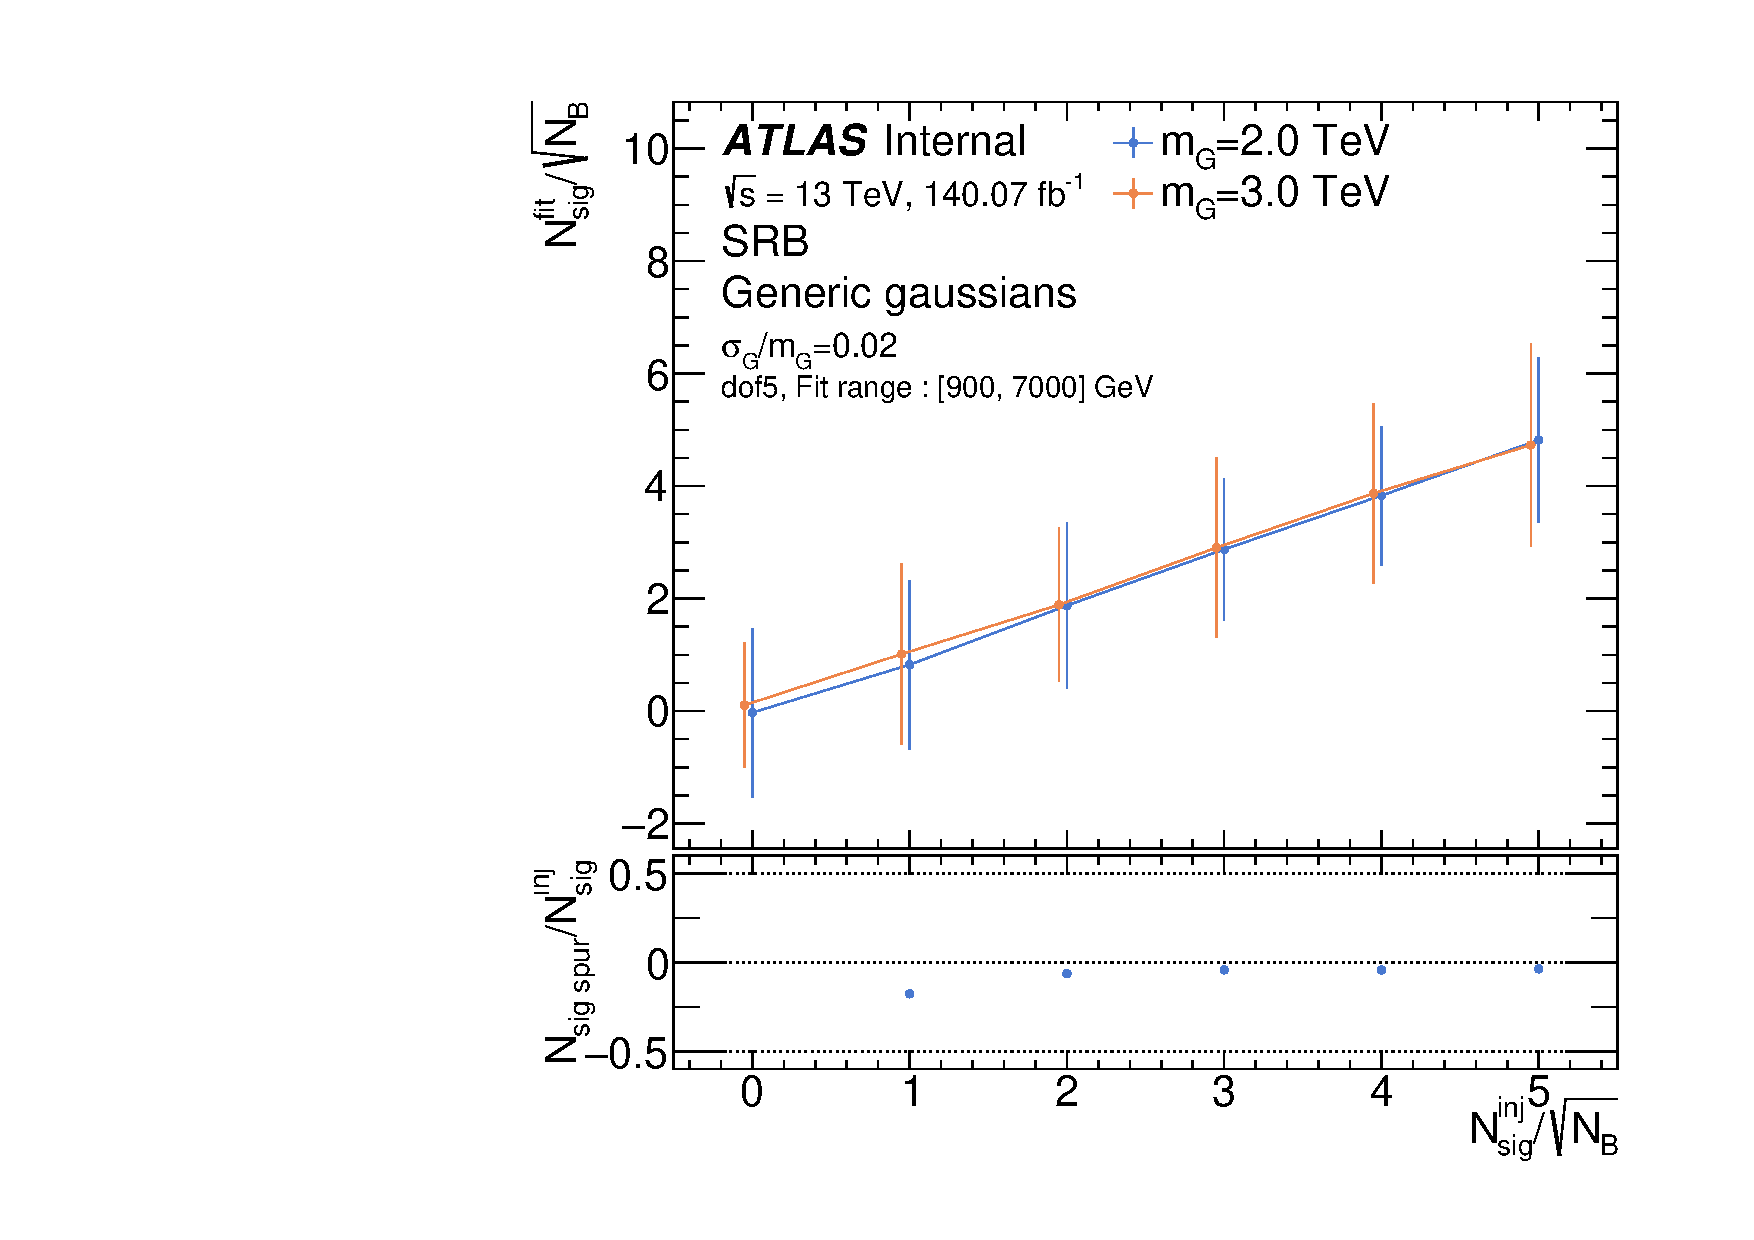
\includegraphics[width=\textwidth]{5_resonances/bkg/modeling/si/toys/SRB/gaus/width0p02/dof5__range_900_7000/plots/can__SigInj__photonjet_Pythia_jfakeisosmooth__gaus__SRB__width0p02__dof5__range_900_7000}
        \caption{\(\sigma_G/\mG = 0.02\).}
    \end{subfigure}
    \hfill
    \begin{subfigure}[h]{0.32\linewidth}
        \centering
        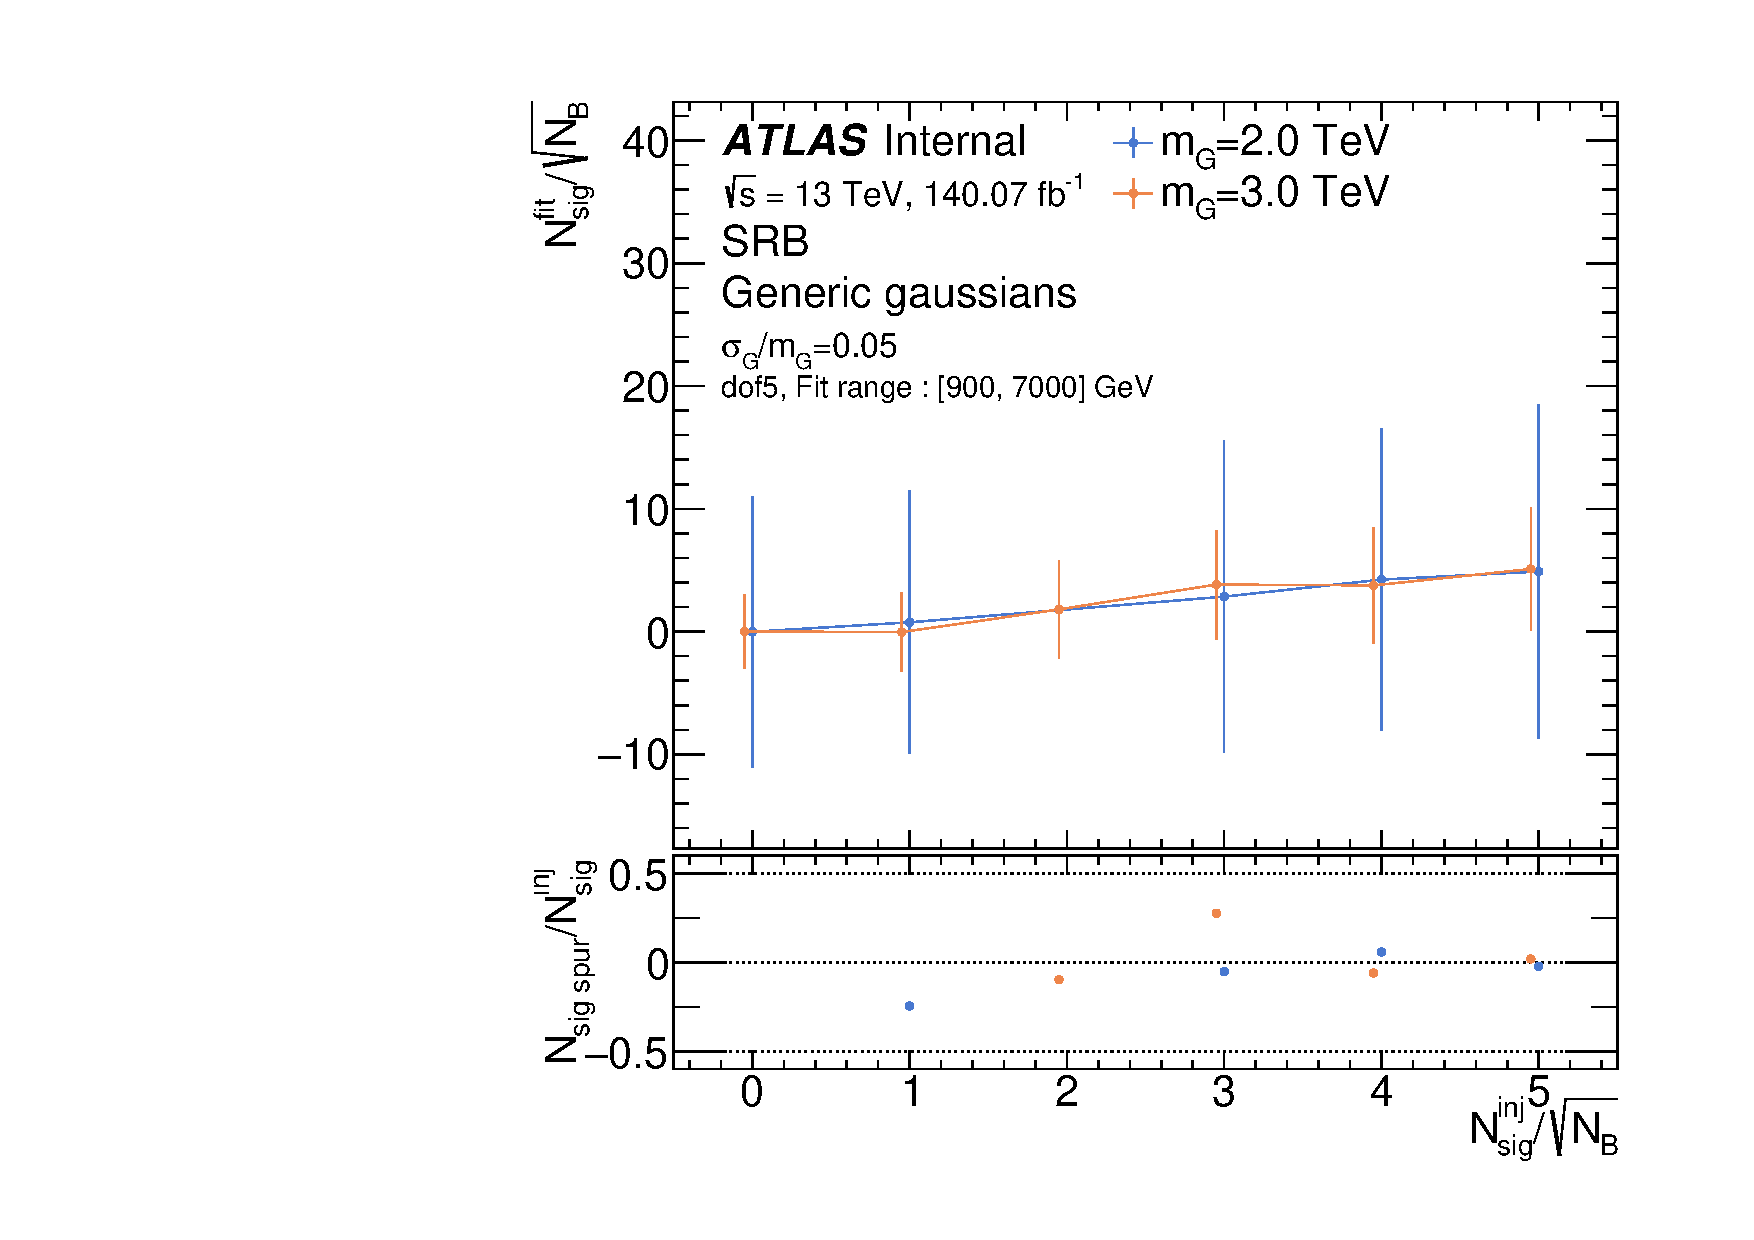
\includegraphics[width=\textwidth]{5_resonances/bkg/modeling/si/toys/SRB/gaus/width0p05/dof5__range_900_7000/plots/can__SigInj__photonjet_Pythia_jfakeisosmooth__gaus__SRB__width0p05__dof5__range_900_7000}
        \caption{\(\sigma_G/\mG = 0.05\).}
    \end{subfigure}
    \hfill
    \begin{subfigure}[h]{0.32\linewidth}
        \centering
        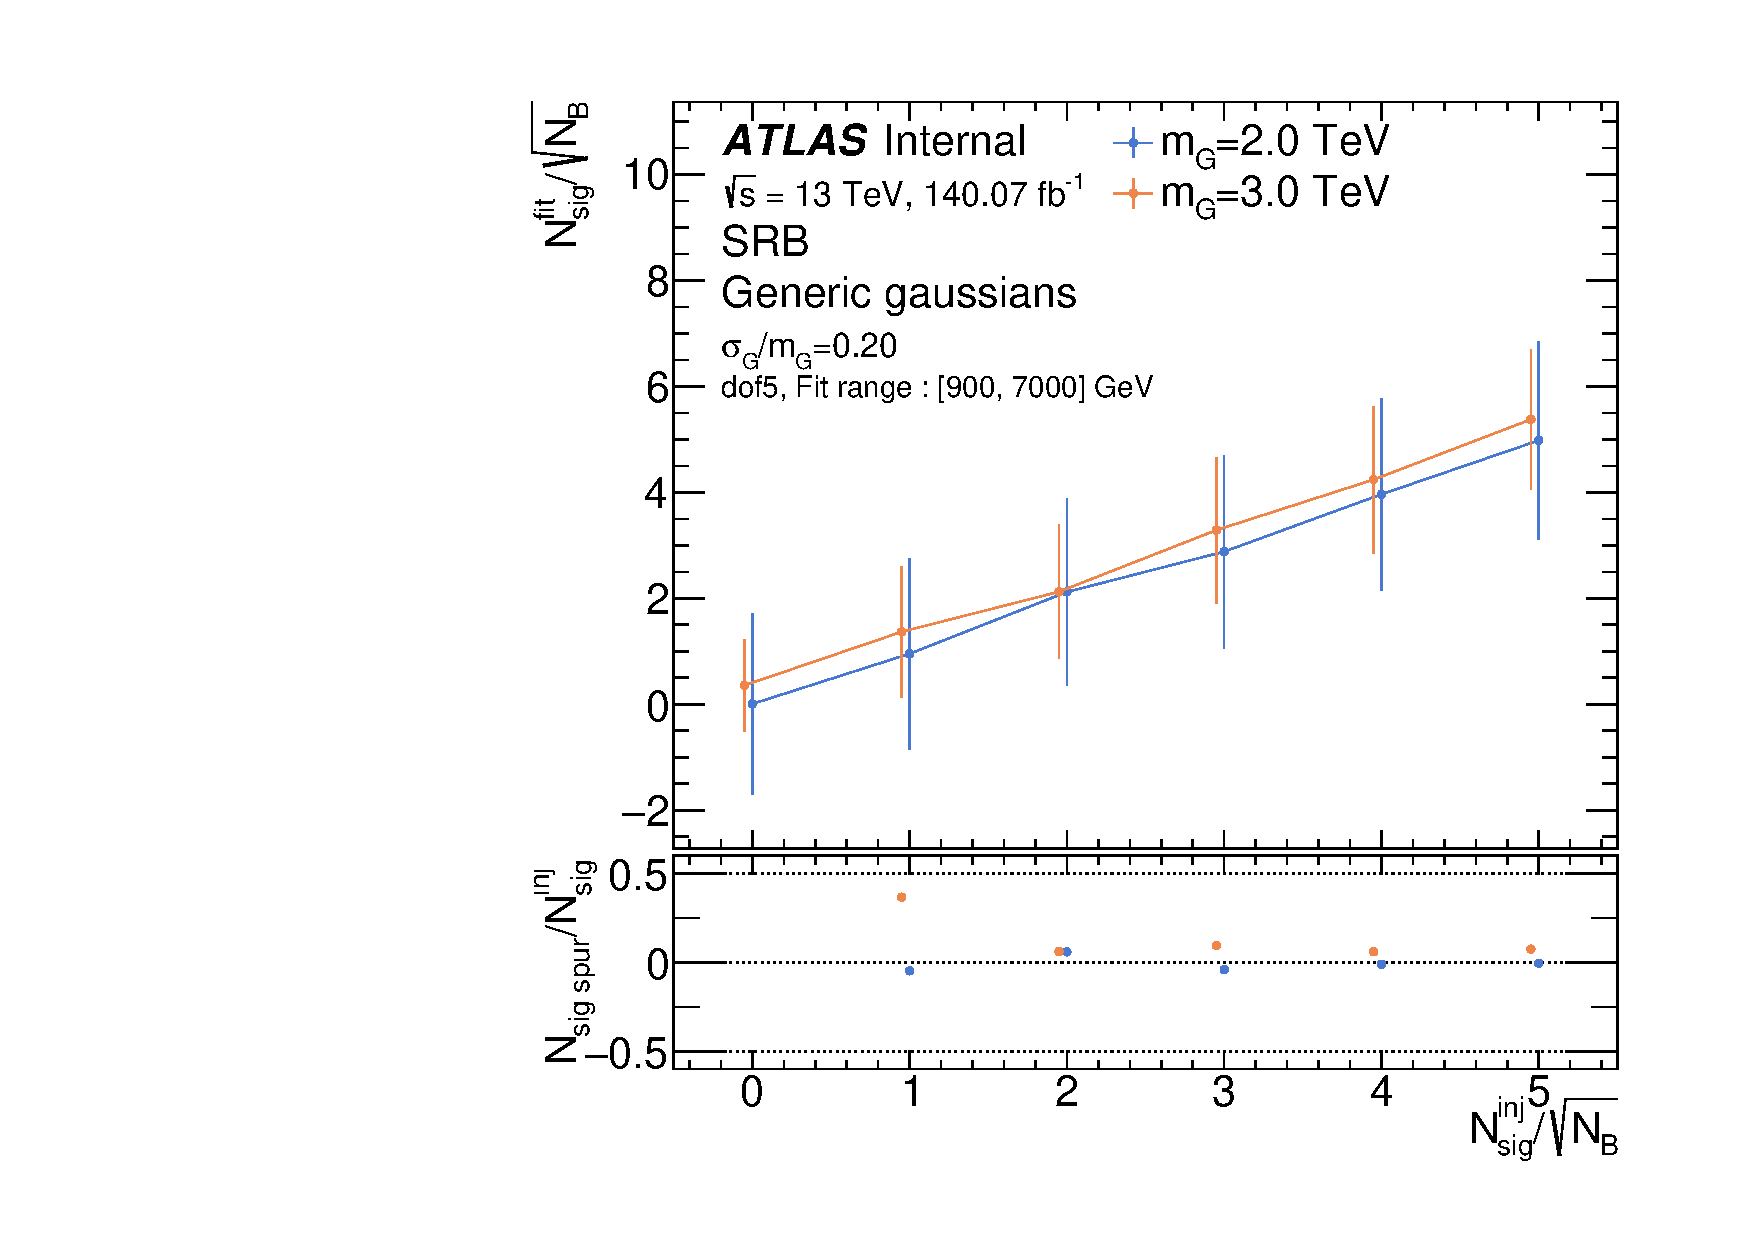
\includegraphics[width=\textwidth]{5_resonances/bkg/modeling/si/toys/SRB/gaus/width0p20/dof5__range_900_7000/plots/can__SigInj__photonjet_Pythia_jfakeisosmooth__gaus__SRB__width0p20__dof5__range_900_7000}
        \caption{\(\sigma_G/\mG = 0.20\).}
    \end{subfigure}
    \caption{Same as \Fig{\ref{fig:si_results:siginj_gaus_SR}} in the SRB region performing fits in the range \(900-7000~\gev\) with the \textit{dpf5} function.}
    \label{fig:si_results:siginj_gaus_SRB}
\end{figure}



\paragraph{Quantum Black Holes}
Similarly to what has been seen for the gaussian signals, in the \acp{QBH} case good linearity is followed by all the considered masses within the fit-range.

\begin{figure}[ht!]
    \centering
    \begin{subfigure}[h]{0.49\linewidth}
        \centering
        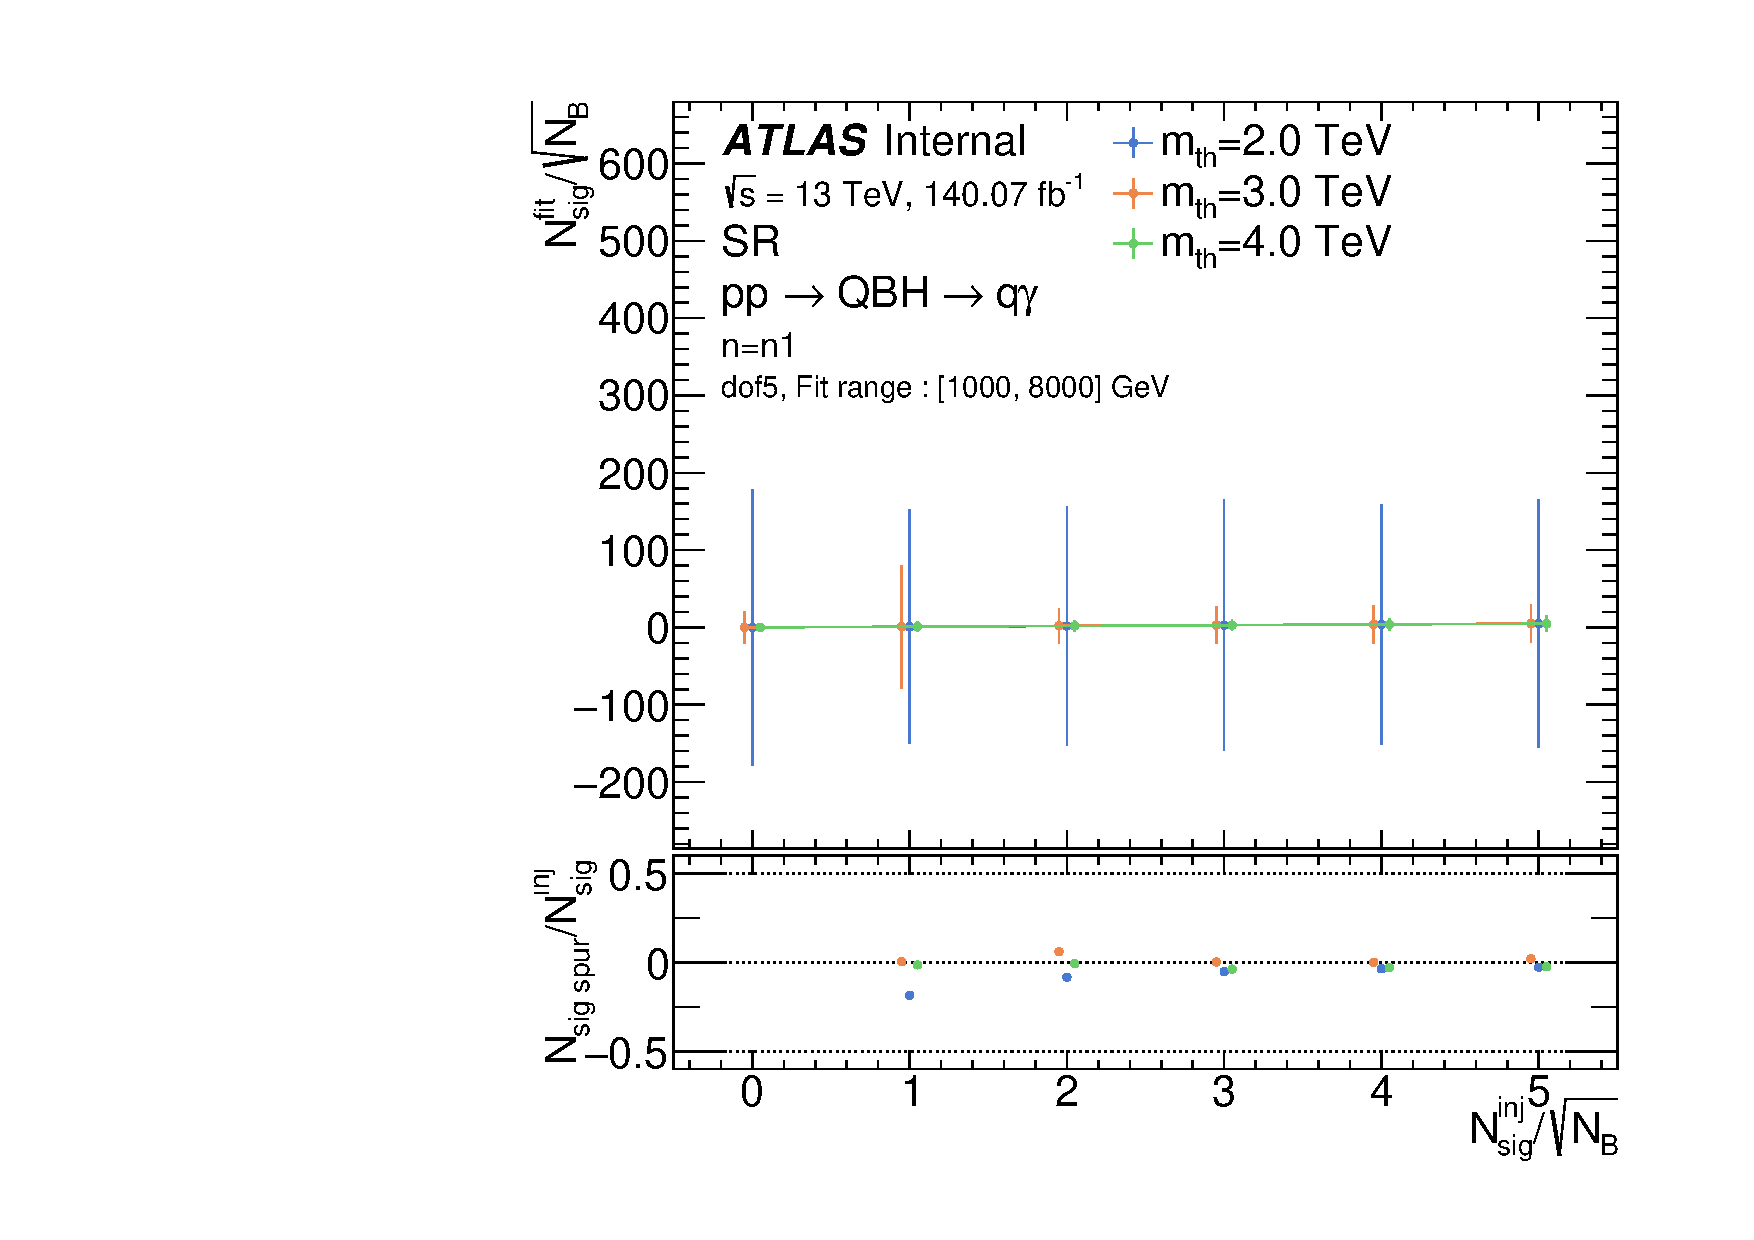
\includegraphics[width=\textwidth]{5_resonances/bkg/modeling/si/toys/SR/QBH/n1/dof5__range_1000_8000/plots/can__SigInj__photonjet_Pythia_jfakeisosmooth__QBH__SR__n1__dof5__range_1000_8000}
        \caption{\(n = 1\) (RS1).}
    \end{subfigure}
    \hfill
    \begin{subfigure}[h]{0.49\linewidth}
        \centering
        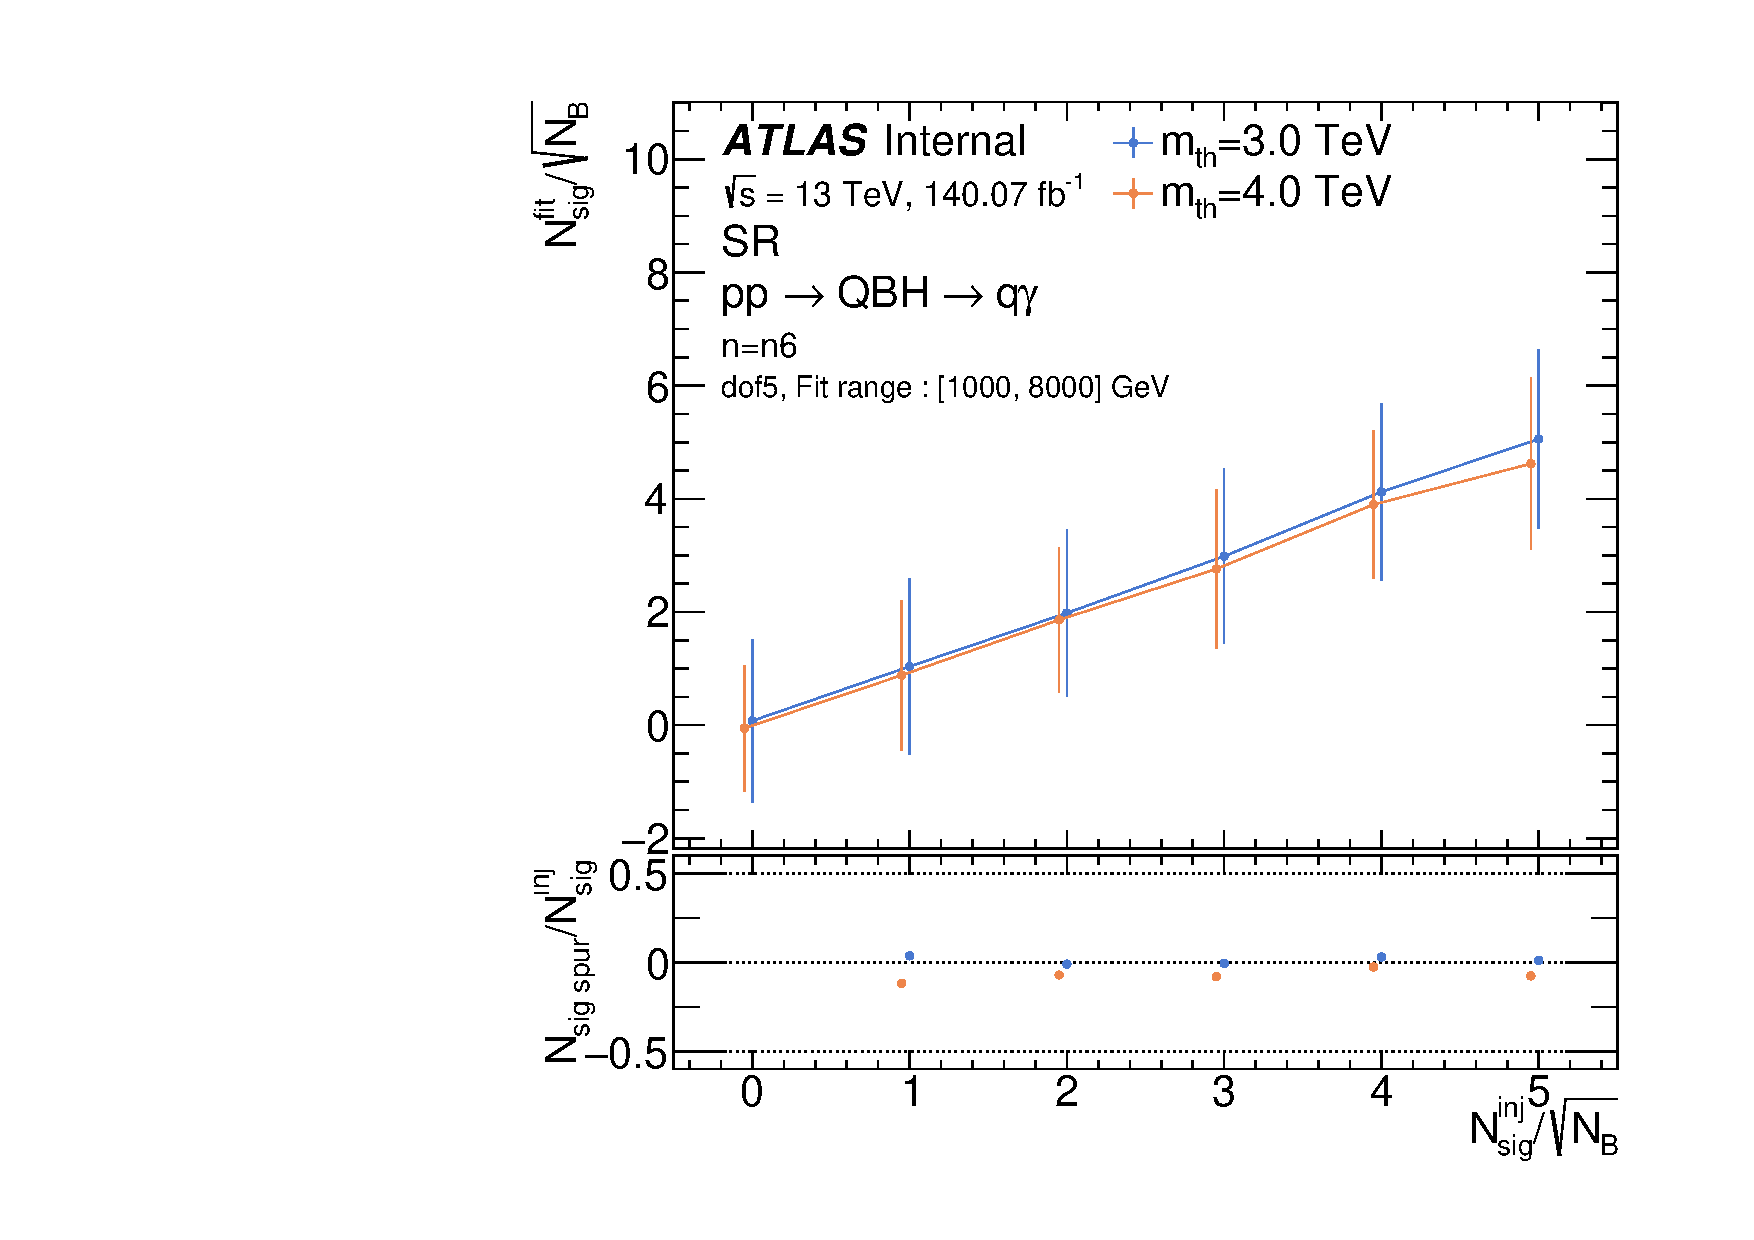
\includegraphics[width=\textwidth]{5_resonances/bkg/modeling/si/toys/SR/QBH/n6/dof5__range_1000_8000/plots/can__SigInj__photonjet_Pythia_jfakeisosmooth__QBH__SR__n6__dof5__range_1000_8000}
        \caption{\(n = 6\) (ADD).}
    \end{subfigure}
    \caption{\ac{SI} tests results using \ac{QBH} signals in the inclusive SR region. The fit is performed in the range \(1000-8000~\gev\) using the \textit{dof5} function.}
    \label{fig:si_results:siginj_QBH_SR}
\end{figure}